
%% Support sites:
%% http://www.michaelshell.org/tex/ieeetran/
%% http://www.ctan.org/tex-archive/macros/latex/contrib/IEEEtran/
%% and
%% http://www.ieee.org/

%%*************************************************************************
%% Legal Notice:
%% This code is offered as-is without any warranty either expressed or
%% implied; without even the implied warranty of MERCHANTABILITY or
%% FITNESS FOR A PARTICULAR PURPOSE! 
%% User assumes all risk.
%% In no event shall IEEE or any contributor to this code be liable for
%% any damages or losses, including, but not limited to, incidental,
%% consequential, or any other damages, resulting from the use or misuse
%% of any information contained here.
%%
%% All comments are the opinions of their respective authors and are not
%% necessarily endorsed by the IEEE.
%%
%% This work is distributed under the LaTeX Project Public License (LPPL)
%% ( http://www.latex-project.org/ ) version 1.3, and may be freely used,
%% distributed and modified. A copy of the LPPL, version 1.3, is included
%% in the base LaTeX documentation of all distributions of LaTeX released
%% 2003/12/01 or later.
%% Retain all contribution notices and credits.
%% ** Modified files should be clearly indicated as such, including  **
%% ** renaming them and changing author support contact information. **
%%
%% File list of work: IEEEtran.cls, IEEEtran_HOWTO.pdf, bare_adv.tex,
%%                    bare_conf.tex, bare_jrnl.tex, bare_jrnl_compsoc.tex
%%*************************************************************************

% *** Authors should verify (and, if needed, correct) their LaTeX system  ***
% *** with the testflow diagnostic prior to trusting their LaTeX platform ***
% *** with production work. IEEE's font choices can trigger bugs that do  ***
% *** not appear when using other class files.                            ***
% The testflow support page is at:
% http://www.michaelshell.org/tex/testflow/



% Note that the a4paper option is mainly intended so that authors in
% countries using A4 can easily print to A4 and see how their papers will
% look in print - the typesetting of the document will not typically be
% affected with changes in paper size (but the bottom and side margins will).
% Use the testflow package mentioned above to verify correct handling of
% both paper sizes by the user's LaTeX system.
%
% Also note that the "draftcls" or "draftclsnofoot", not "draft", option
% should be used if it is desired that the figures are to be displayed in
% draft mode.
%
\documentclass[conference]{IEEEtran}
% If IEEEtran.cls has not been installed into the LaTeX system files,
% manually specify the path to it like:
% \documentclass[conference]{../sty/IEEEtran}





% Some very useful LaTeX packages include:
% (uncomment the ones you want to load)



% *** CITATION PACKAGES ***
%
\usepackage{cite}
% cite.sty was written by Donald Arseneau
% V1.6 and later of IEEEtran pre-defines the format of the cite.sty package
% \cite{} output to follow that of IEEE. Loading the cite package will
% result in citation numbers being automatically sorted and properly
% "compressed/ranged". e.g., [1], [9], [2], [7], [5], [6] without using
% cite.sty will become [1], [2], [5]--[7], [9] using cite.sty. cite.sty's
% \cite will automatically add leading space, if needed. Use cite.sty's
% noadjust option (cite.sty V3.8 and later) if you want to turn this off.
% cite.sty is already installed on most LaTeX systems. Be sure and use
% version 4.0 (2003-05-27) and later if using hyperref.sty. cite.sty does
% not currently provide for hyperlinked citations.
% The latest version can be obtained at:
% http://www.ctan.org/tex-archive/macros/latex/contrib/cite/
% The documentation is contained in the cite.sty file itself.






% *** GRAPHICS RELATED PACKAGES ***
%
\ifCLASSINFOpdf
   \usepackage[pdftex]{graphicx}
  % declare the path(s) where your graphic files are
  % \graphicspath{{../pdf/}{../jpeg/}}
  % and their extensions so you won't have to specify these with
  % every instance of \includegraphics
  % \DeclareGraphicsExtensions{.pdf,.jpeg,.png}
\else
  % or other class option (dvipsone, dvipdf, if not using dvips). graphicx
  % will default to the driver specified in the system graphics.cfg if no
  % driver is specified.
  % \usepackage[dvips]{graphicx}
  % declare the path(s) where your graphic files are
  % \graphicspath{{../eps/}}
  % and their extensions so you won't have to specify these with
  % every instance of \includegraphics
  % \DeclareGraphicsExtensions{.eps}
\fi
% graphicx was written by David Carlisle and Sebastian Rahtz. It is
% required if you want graphics, photos, etc. graphicx.sty is already
% installed on most LaTeX systems. The latest version and documentation can
% be obtained at: 
% http://www.ctan.org/tex-archive/macros/latex/required/graphics/
% Another good source of documentation is "Using Imported Graphics in
% LaTeX2e" by Keith Reckdahl which can be found as epslatex.ps or
% epslatex.pdf at: http://www.ctan.org/tex-archive/info/
%
% latex, and pdflatex in dvi mode, support graphics in encapsulated
% postscript (.eps) format. pdflatex in pdf mode supports graphics
% in .pdf, .jpeg, .png and .mps (metapost) formats. Users should ensure
% that all non-photo figures use a vector format (.eps, .pdf, .mps) and
% not a bitmapped formats (.jpeg, .png). IEEE frowns on bitmapped formats
% which can result in "jaggedy"/blurry rendering of lines and letters as
% well as large increases in file sizes.
%
% You can find documentation about the pdfTeX application at:
% http://www.tug.org/applications/pdftex





% *** MATH PACKAGES ***
%
%\usepackage[cmex10]{amsmath}
% A popular package from the American Mathematical Society that provides
% many useful and powerful commands for dealing with mathematics. If using
% it, be sure to load this package with the cmex10 option to ensure that
% only type 1 fonts will utilized at all point sizes. Without this option,
% it is possible that some math symbols, particularly those within
% footnotes, will be rendered in bitmap form which will result in a
% document that can not be IEEE Xplore compliant!
%
% Also, note that the amsmath package sets \interdisplaylinepenalty to 10000
% thus preventing page breaks from occurring within multiline equations. Use:
%\interdisplaylinepenalty=2500
% after loading amsmath to restore such page breaks as IEEEtran.cls normally
% does. amsmath.sty is already installed on most LaTeX systems. The latest
% version and documentation can be obtained at:
% http://www.ctan.org/tex-archive/macros/latex/required/amslatex/math/





% *** SPECIALIZED LIST PACKAGES ***
%
\usepackage{algorithm2e}
% algorithmic.sty was written by Peter Williams and Rogerio Brito.
% This package provides an algorithmic environment fo describing algorithms.
% You can use the algorithmic environment in-text or within a figure
% environment to provide for a floating algorithm. Do NOT use the algorithm
% floating environment provided by algorithm.sty (by the same authors) or
% algorithm2e.sty (by Christophe Fiorio) as IEEE does not use dedicated
% algorithm float types and packages that provide these will not provide
% correct IEEE style captions. The latest version and documentation of
% algorithmic.sty can be obtained at:
% http://www.ctan.org/tex-archive/macros/latex/contrib/algorithms/
% There is also a support site at:
% http://algorithms.berlios.de/index.html
% Also of interest may be the (relatively newer and more customizable)
% algorithmicx.sty package by Szasz Janos:
% http://www.ctan.org/tex-archive/macros/latex/contrib/algorithmicx/





% *** ALIGNMENT PACKAGES ***
%
%\usepackage{array}
% Frank Mittelbach's and David Carlisle's array.sty patches and improves
% the standard LaTeX2e array and tabular environments to provide better
% appearance and additional user controls. As the default LaTeX2e table
% generation code is lacking to the point of almost being broken with
% respect to the quality of the end results, all users are strongly
% advised to use an enhanced (at the very least that provided by array.sty)
% set of table tools. array.sty is already installed on most systems. The
% latest version and documentation can be obtained at:
% http://www.ctan.org/tex-archive/macros/latex/required/tools/


%\usepackage{mdwmath}
%\usepackage{mdwtab}
% Also highly recommended is Mark Wooding's extremely powerful MDW tools,
% especially mdwmath.sty and mdwtab.sty which are used to format equations
% and tables, respectively. The MDWtools set is already installed on most
% LaTeX systems. The lastest version and documentation is available at:
% http://www.ctan.org/tex-archive/macros/latex/contrib/mdwtools/


% IEEEtran contains the IEEEeqnarray family of commands that can be used to
% generate multiline equations as well as matrices, tables, etc., of high
% quality.


%\usepackage{eqparbox}
% Also of notable interest is Scott Pakin's eqparbox package for creating
% (automatically sized) equal width boxes - aka "natural width parboxes".
% Available at:
% http://www.ctan.org/tex-archive/macros/latex/contrib/eqparbox/





% *** SUBFIGURE PACKAGES ***
\usepackage[tight,footnotesize]{subfigure}
% subfigure.sty was written by Steven Douglas Cochran. This package makes it
% easy to put subfigures in your figures. e.g., "Figure 1a and 1b". For IEEE
% work, it is a good idea to load it with the tight package option to reduce
% the amount of white space around the subfigures. subfigure.sty is already
% installed on most LaTeX systems. The latest version and documentation can
% be obtained at:
% http://www.ctan.org/tex-archive/obsolete/macros/latex/contrib/subfigure/
% subfigure.sty has been superceeded by subfig.sty.



%\usepackage[caption=false]{caption}
%\usepackage[font=footnotesize]{subfig}
% subfig.sty, also written by Steven Douglas Cochran, is the modern
% replacement for subfigure.sty. However, subfig.sty requires and
% automatically loads Axel Sommerfeldt's caption.sty which will override
% IEEEtran.cls handling of captions and this will result in nonIEEE style
% figure/table captions. To prevent this problem, be sure and preload
% caption.sty with its "caption=false" package option. This is will preserve
% IEEEtran.cls handing of captions. Version 1.3 (2005/06/28) and later 
% (recommended due to many improvements over 1.2) of subfig.sty supports
% the caption=false option directly:
%\usepackage[caption=false,font=footnotesize]{subfig}
%
% The latest version and documentation can be obtained at:
% http://www.ctan.org/tex-archive/macros/latex/contrib/subfig/
% The latest version and documentation of caption.sty can be obtained at:
% http://www.ctan.org/tex-archive/macros/latex/contrib/caption/




% *** FLOAT PACKAGES ***
%
%\usepackage{fixltx2e}
% fixltx2e, the successor to the earlier fix2col.sty, was written by
% Frank Mittelbach and David Carlisle. This package corrects a few problems
% in the LaTeX2e kernel, the most notable of which is that in current
% LaTeX2e releases, the ordering of single and double column floats is not
% guaranteed to be preserved. Thus, an unpatched LaTeX2e can allow a
% single column figure to be placed prior to an earlier double column
% figure. The latest version and documentation can be found at:
% http://www.ctan.org/tex-archive/macros/latex/base/



%\usepackage{stfloats}
% stfloats.sty was written by Sigitas Tolusis. This package gives LaTeX2e
% the ability to do double column floats at the bottom of the page as well
% as the top. (e.g., "\begin{figure*}[!b]" is not normally possible in
% LaTeX2e). It also provides a command:
%\fnbelowfloat
% to enable the placement of footnotes below bottom floats (the standard
% LaTeX2e kernel puts them above bottom floats). This is an invasive package
% which rewrites many portions of the LaTeX2e float routines. It may not work
% with other packages that modify the LaTeX2e float routines. The latest
% version and documentation can be obtained at:
% http://www.ctan.org/tex-archive/macros/latex/contrib/sttools/
% Documentation is contained in the stfloats.sty comments as well as in the
% presfull.pdf file. Do not use the stfloats baselinefloat ability as IEEE
% does not allow \baselineskip to stretch. Authors submitting work to the
% IEEE should note that IEEE rarely uses double column equations and
% that authors should try to avoid such use. Do not be tempted to use the
% cuted.sty or midfloat.sty packages (also by Sigitas Tolusis) as IEEE does
% not format its papers in such ways.





% *** PDF, URL AND HYPERLINK PACKAGES ***
%
%\usepackage{url}
% url.sty was written by Donald Arseneau. It provides better support for
% handling and breaking URLs. url.sty is already installed on most LaTeX
% systems. The latest version can be obtained at:
% http://www.ctan.org/tex-archive/macros/latex/contrib/misc/
% Read the url.sty source comments for usage information. Basically,
% \url{my_url_here}.





% *** Do not adjust lengths that control margins, column widths, etc. ***
% *** Do not use packages that alter fonts (such as pslatex).         ***
% There should be no need to do such things with IEEEtran.cls V1.6 and later.
% (Unless specifically asked to do so by the journal or conference you plan
% to submit to, of course. )


% correct bad hyphenation here
\hyphenation{op-tical net-works semi-conduc-tor}


\begin{document}
%
% paper title
% can use linebreaks \\ within to get better formatting as desired
\title{Jaguar Lite Point Tracking}

\author{\IEEEauthorblockN{Lauren Lieu}
\IEEEauthorblockA{
Department of Engineering\\
Harvey Mudd College\\
Email: llieu@g.hmc.edu}
\and
\IEEEauthorblockN{Joshua Vasquez}
\IEEEauthorblockA{Department of Engineering\\
Harvey Mudd College\\
Email: jvasquez@g.hmc.edu}
}

% make the title area
\maketitle
{\flushleft March 5, 2013}\\
\IEEEpeerreviewmaketitle

\begin{abstract}
This paper describes the implementation of point tracking for the \emph{Jaguar Lite Mobile Robot Platform}. Motion control of the autonomous vehicle is achieved using a Proportional-Integral-Derivative controller. In both simulation and hardware mode, the control law parameters and control gains have been tuned to demonstrate stable, precise motion towards desired goal states.
\end{abstract} 

\section{Introduction}
Autonomous localization is a critical step in algorithm development on robotic platforms.  Answering the simple question: ``Where am I in
a known environment?'' is a task that can be answered using external sensors.
However, before such a question can be addressed, the designers must first
understand the limitations of the robot's odometry sensors which form the basis
 of estimating the robot's pose in a given environment. In the following paper, 
we the designers carry out a series of experiments necessary to characterize 
the accuracy of the incremental encoders on the Jaguar Lite platform, and our findings confirm a linear relationship between 
odometry-based localization and actual robot position for several types of terrain. 

We characterize both the robot's linear displacement and angular 
displacement relative to it's true displacement measured through the use of 
external measuring equipment.

\subsection{Hardware Platform}
The hardware platform of choice is a Jaguar Lite autonomous vehicle, sourced 
by Dr. Robot.  This differential-drive platform is fairly rugged, and 
features a suite of sensory inputs: a 9 DOF Inertial measurement unit (IMU), 
two rotary encoders, a 240$^{\circ}$ field-of-view laser range finder, and an
onboard webcam \cite{Dr.RobotWebsite}.  With a wireless wifi interface, the 
designer can implement navigation algorithms in \emph{C\#} within Microsoft Visual Studio to communicate with the Jaguar platform. Most importantly, the platform can  be driven both 
indoors and outdoors. 


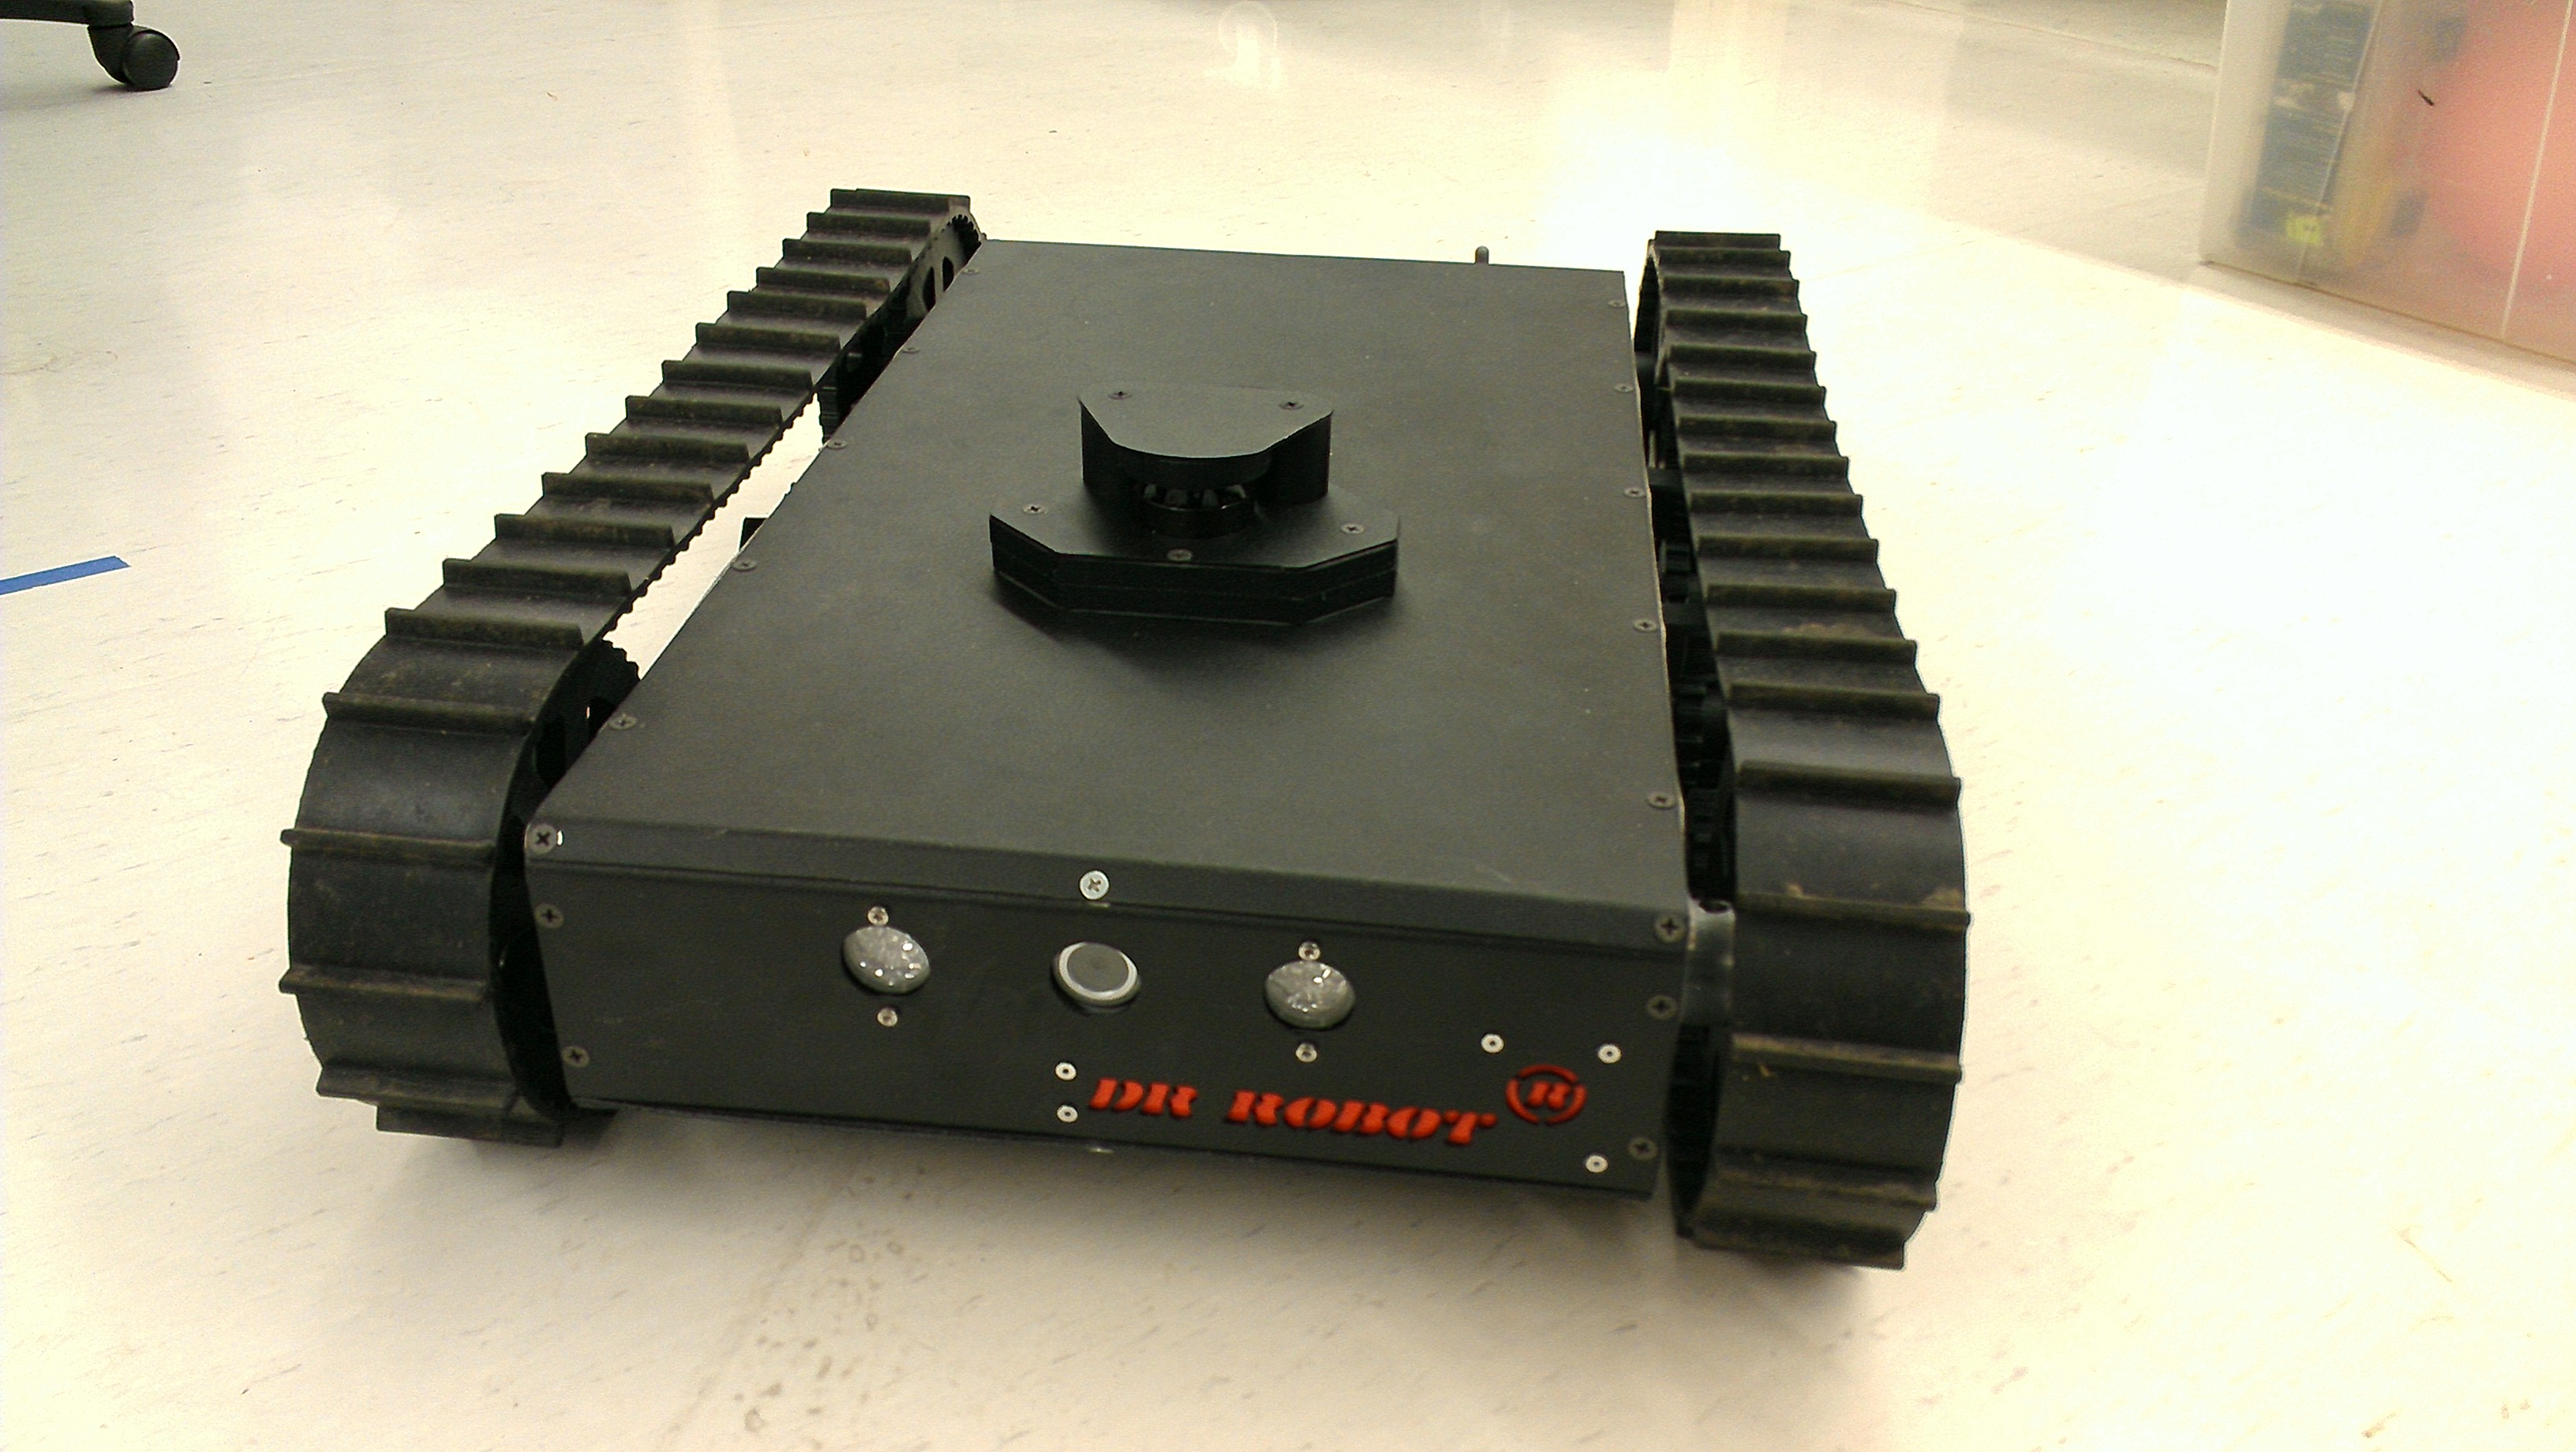
\includegraphics[width = 3in]{jaguarLite.png}\\
\textbf{Figure 1.}

\subsection{Terminology}
This paper refers to specific definitions and usage of the following terms:

\begin{itemize}
\item \noindent \textbf{Pose} represents the robot's position: $[x,y,\theta]$ relative to a 
coordinate frame fixed to the environment that the robot navigates.

\item \noindent\textbf{Linear drift} for a given axis is defined to be the difference between the 
robot's true displacement and the robot's calculated displacement from encoder
measurements.

\item \noindent\textbf{Angular drift}  is the difference between the robot's true 
angular offset (relative to a fixed coordinate frame) and its 
calculated angular offset relative to its starting position.
\end{itemize}

A measurement is characterized as \emph{true} if it is the measurement calculated 
in the environment with external measuring tools, such as a meterstick or
compass. Another measurement from on-board sensors may be considered true if and only if it corresponds to the localization measurements in the global coordinate frame.
 
\section{Method}
\subsection{Motion Model}
\begin{equation}
\rho = \sqrt{\Delta x^2 + \Delta y^2}
\end{equation}
\begin{equation}
\alpha = -\theta + atan2(\Delta y, \Delta x)
\end{equation}
\begin{equation}
\beta = -\theta -\alpha
\end{equation}
Assuming the robot is travelling on a circular arc of constant radius, we can apply basic circle geometry to calculate the distance traveled $\Delta s$ and the change in orientation $\Delta\theta$ of each tread of the Jaguar Lite robot for time step $\Delta t$. These changes in displacement are within the local coordinate frame of the robot. To convert the position change of the robot into the global coordinate frame, we assume that the robot's motion is small in a given time step. As a result, the robot's trajectory can be approximated to be a straight path, and using trigonometry we derived the following equations to determine the change in position within a global coordinate frame, where $L$ is the radius of the robot.

\subsection{Experiments Performed}
\subsubsection{Linear Drift}
The robot localizes itself from odometry measurements by calculating the linear
 distance travelled from its last distance.  In reality, such a calculation is 
an approximation, subject to drift.  
With the given instrumentation, we chose to measure the linear drift along the 
x-axis, by measuring the robot's true x-displacement and comparing it to the 
odometry-calculated x-displacement.  An illustration of the measurement is shown
in figure [xxxxx].



\includegraphics[width = 3.2in]{measurements.png}
\textbf{fig 2}

To characterize the Jaguar Lite's pose drift, we conducted a series 
of measurements to compare the robot's odometry-deduced pose with its true
 pose given by its location in the global coordinate frame.  At the high level, the 
robot, upon reset, places itself in the origin of the map.  We define the 
robot's starting position as the origin of the true map as well, shown in figure [xxxx].



\includegraphics[width = 3.2in]{origin.png}
\textbf{fig 3}

\subsubsection{Angular Drift}


\section{Results}
\subsection{Linear Drift}
From three averaged datasets, we characterized the odometry sensor accuracy on 
two environments, both grass and concrete. The graphs in figure [xxxx] and [xxxx] 
display the \emph{True X Displacement} against the \emph{Odometry-Calculated Displacement}.
In addition, the ideal Odometry Measurement has also been plotted for reference, 
where we define ideal measurement to be the case where the true displacement
and the perceived displacement match, such that the ideal slope of plotted odometry and external measurements is unity.


\includegraphics[width = 3.25in]{grass_avg.png}
\textbf{fig 4}


\includegraphics[width = 3.25in]{concrete_avg.png}
\textbf{fig 5}

The linear fit for the average grass drift was $r^2 = 1.0000$, and the linear fit for 
the average concrete drift was $r^2 = 0.9998$, indicating that a line is a good fit 
for both datasets.  
From both plots on the grass and the concrete forward-driving data, we can 
see a clear deviation from the ideal odometry value of the encoders.  This 
error is more clearly illustrated in the following graphs, which plot the error
 as a function of odometry measurement.  (Note 
the units of the y-axis.)  


\includegraphics[width=3.25in]{grass_error.png}
\textbf{fig 6}


\includegraphics[width=3.25in]{concrete_error.png}
\textbf{fig 7}

Thus, as the overall distance travelled (as recorded by the odometry) increases, 
the overall error increases in a linear fashion. Furthermore, we can see that 
slope of the error graph is approximately an order of magnitude smaller than that of 
the corresponding \emph{Distance vs Odometry} plot. 


Additionally, four trials of data were collected on a tile surface wherein the 
Jaguar Lite travelled either forward or backward along the tile surface.  
A linear fit of the data produced a fit value of $r^2 = 1.0000$, and the 
results are depicted in the following graphs. 

\includegraphics[width=3.25in]{tiles_average.png}
\textbf{fig 8}



\includegraphics[width=3.25in]{tiles_error.png}
\textbf{fig 9}

Thus, the Jaguar Lite also demonstrates a linear error offset from forward and 
backward motion on tiled surfaces. An important note about this final dataset, 
however, is that the Jaguar Lite's forward motion is determined to be 
characteristically identical to its reverse motion. 

\subsection{Angular Drift}
  To characterize angular drift the robot rotated through several 
iterations of angles, and both the true angle was recorded (with a 
compass) as well as the measured angle according to the robot's odometry. The 
results of the raw data collection are plotted below as true rotations (in 
radians) versus rotation measurements from the wheel odometry.



\includegraphics[width=3.25in]{tiles_rotation.png}
\textbf{fig 10}



\includegraphics[width=3.25in]{tiles_rotation_error.png}
\textbf{fig 11}

\section{Conclusion}
The results of this odometry error characterization are promising for future 
work on the Jaguar Lite robotic platform.  With additional 
analysis (i.e: more data-collection over longer distances), we may be able 
to throroughly characterize the drift for the robot's pose and calculate an
error-correction function which the robot can implement to reduce 
error from its odometry measurement. From the data collected, we can 
indeed produce error functions from which the robot can better estimate its 
true pose; however, more data-collection is necessary to verify the constants 
associated with the linear fit.  Additional testing is necessary, especially for grassy terrain since data-collection was performed on the same patch of grass, 
potentially changing the characteristics of the grass surface with each 
measurement.


\subsection{Linear Drift}
We successfully characterized the odometry error of the Jaguar Lite for straight trajectors. There is a linear relationship between odometry-based localization and the actual position of the robot in the global coordinate frame. The error in the robot's \emph{[x,y]} pose estimation for three surfaces: tile, grass, and concrete ranges from eight to ten percent.

\subsection{Angular Drift}
Overall, we have concluded that for tile surfaces, error does indeed linearly increase as the number 
of measured rotations increases.  We expect that the error can also be fitted
with a linear function for other surfaces; however, to generate an actual function, 
more data collection is necessary. 

Furthermore, the order of magnitude over which this linear drift is linear must be
explicitly stated to be on the order of rotations.  Thus, we cannot generalize that
because the error behaves linearly overall for 1,2, or even 10 rotations, so too must 
the error function be linear on the order of values less than a rotation.  While
such a conclusion is plausible, more data is needed to verify such a result. 


\section*{Acknowledgment}


The authors would like to thank Professor Christopher Clark for 
establishing a software framework on which we can 
develop our algorithms, as well as fellow collaborators Taylor Peterson, Hannah
Kastein, Samuel Yim, and Benjamin Chasnov for their mutual effort collecting
additional data.




\begin{thebibliography}{1}

\bibitem{LaboratoryExercise1}%IEEEhowto:kopka}
\begin{verbatim}
http://newwww.hmc.edu/lair/E190Q/
E190Q-Lab01-IntroToTheJaguar.pdf
\end{verbatim}

\bibitem{Dr.RobotWebsite}
\begin{verbatim}
http://jaguar.drrobot.com/specification_lite.asp
\end{verbatim}

\bibitem{PDFOfEquations}
\begin{verbatim}
http://newwww.hmc.edu/lair/E190Q/E190Q
-Lecture03-Odometry.pdf
\end{verbatim}

\bibitem{Probabilistic}
Thrun, Sebastian, et. all. \emph{Probabilistic Robotics}
2005, The MIT Press.


\end{thebibliography}




% that's it, dude!
\end{document}


